\chapter{Preliminaries and Problem Setup}
\label{sec:preliminariesProblem}


In the following chapter, the problem setup handled by the Master Thesis will be explained.
Further, preliminaries regarding assumptions and other decisions are defined.

\section{Tomographic reconstruction problem}
\label{sec:reconstructionProblemCT}
Tomographic reconstruction\cite{tomographicReconstruction} is a popular inverse problem \cite{tomographicReconstruction}. 
The aim is to reconstruct an object $x$ from its observed projections $\mathcal{P}=[\rho_0, \rho_1, \dots, \rho_N]$.
More formally, the aim is to recover some density function $f$ from overserved samples $y$, taken from the line-integral $\rho(\cdot)$.

The problem can be defined as a two-dimensional (2D) problem but also as a three-dimensional (3D) problem. 
In the following, we focus on the 2D case.
In 2D, also called classical tomography reconstruction problem, the underlying density function is in two dimensions and the measurement lines lie on a plane.

The problem automatically gets harder, if we deal with incomplete datasets (subset of measured lines, limited angle data) but also with noisy observations.

\paragraph{Classical tomography reconstruction}

First of all, lets define the line integral $\rho$ of our unknown density function $f$ in the classical case:

\begin{equation}
    \begin{aligned}
        y_i &= \rho_i (\theta_i, s_i)
        \rho(\theta, s)   &=  R f(\theta, s) \\
        R f(\theta, s) &=  \int_{-\infty}^{\infty} f(x(z), y(z)) dz \\
        &= \int_{-\infty}^{\infty} f((z \sin \theta + s \cos \theta), (-z \cos \theta + s \sin \theta)) dz \\
    \end{aligned}
\end{equation}

where $\rho$ is the line integral of the density function $f$, $\theta$ the projection angle and $s$ the distance from the origin.

In the 2D case, the line integral corresponds to the Radon-Transform $Rf$
With the 2D Radon transform, we can map the density function $f$ to the sinogram $\rho$. 

\paragraph{Filter Backprojection}
\label{sec:filterBackProjection}
Filter Backprojection (FBP) is a reconstruction method, typically used in classical tomography reconstruction.
It allows to solve for $\rho$ and is equivalent to the inverse of the Radon Transform
and is related to the Fourier transform. 

Basically, it maps sinograms of $\rho$ back to the density function $f$.

\begin{equation}
    f(x) = \int_{0}^{\pi} Rf(\theta, s) |_{s=x \cdot (- \sin \theta, cos \theta) } d \theta
\end{equation}

The disadvantage of the algorithm is, that it only works for complete data and without noise
and needs adjustments when dealing with such scenarios. 

\section{Cryo-EM}
Similar to tomographic reconstruction, there is the cryo-EM reconstruction problem\cite{cryoEmMath}.
It can be seen as a 3D reconstruction problem as the original object $x$ to be reconstructed is in 3D.

During observation process, the object will be frozen, which results in a random rotation, and from this intermediate state 
projections $\mathcal{P}=[\rho_0, \rho_1, \dots, \rho_N]$ are observed.

More formally, the aim is to recover some density function $f$ from overserved samples $y$, taken from 
randomly rotated, projected 2D samples.

The two problem are highly related, but the cryo-EM reconstruct is even harder than tomographic reconstruction.
During CT observation, the patient is asked to not move and therefore, the angles of projection is known, whereas
in cryo-EM this information will be lost during the freezing process.
Secondly, the high level of noise makes cryo-EM much more challenging regarding tomographic reconstruction.

\begin{equation}
    \label{eg:cryoEmSimple}
    y_i = \Pi_z \left( R_{\theta} x) \right) + noise,
\end{equation}

where $R_{\theta}$ is a 3D rotation and $\theta \in SO(3)$, $\Pi_z$ the tomographic projection.

\paragraph{Extended formula:} 
The equation~\ref{eg:cryoEmSimple} is a simplified version of the cryo-EM reconstruction problem.
First of all, the point spread function (PSF) of the microscope is not taken into account.
Moreover, due to structural variety in the molecule, the underlying object $x$ is not the same 
for every observation but can be seen as a random signal from an unknown distribution defined over all possible molecules structures.

The extended version can be defined as follows
\begin{equation}
    \label{eg:cryoEmExtended}
    y_i = h_i * \Pi_z \left( R_{\theta} x_i) \right) + noise,
\end{equation}

where $h_i$ is the PSF of the microscope and $*$ defines the convolution.

\section{General form}
\textbf{TODO:}
We don't observe $y_i \in L^2$ but $y_i = y_i(\Delta) $, with $\Delta \subset (R^{D-1})^N$ a grid containing $N$ points. 

As the tomographic reconstruction and the cryo-EM reconstruction are rather similar, 
the aim of the Master Thesis will be to design an algorithm, that can be applied in both scenarios.

Therefore, a general form of the two problem will be defined in the following.
First of all, we define $x \in L^2(\Omega)$, where $L^2$ is the Lebesgue space and $\Omega$
is the sample space $\Omega \subset \mathbb{R}^D$, where $D$ is the dimension of the sample space. 
Further we define $\tilde{\Omega} \subset \mathbb{R}^{D-1}$.


\begin{equation}
    \begin{aligned}
        y_i &= A(x, \theta) + \eta \\
    \end{aligned}
\end{equation}

where $y_i$ is the observed sample, $x$ our original object, $A$ a non-linear operator 
$A: x \in L^2(\Omega) \rightarrow \tilde{x} \in L^2(\tilde{\Omega})$ and $\eta ~ \mathcal{N}(O, \sigma^2 I)$ gaussian noise.

\paragraph{Classical tomography reconstruction:}

For classical tomography, the parameters can be defined with $D=2$ and $\theta \in SO(1)$.
Further, $A(\cdot)$ can be defined as the Radon transform. 
A distance measure between samples can be set up by using the l2-norm $\norm{y_i - y_j}$.

\paragraph{Cryo-Em reconstruction:}
For classical tomography, the parameters can be defined with $D=3$ and $\theta \in SO(3)$.
Further, $A(\cdot)$ can be defined as $\Pi_z \left( R_{\theta} x) \right)$ 
where $R_{\theta}$ is a 3D rotation and $\theta \in SO(3)$, $\Pi_z$ the tomographic projection.
As the samples are drawn with some random 3D rotation and then will be projected, it can 
happen that two samples are equivalent up to an 2D rotation. 
Consider a first example $y_1$, which has no 3D rotation at all and 
a second sample $y_2$ with a rotation only in in x-y plane by 45°.
The two samples have a defined in-plane rotation $g$, such that $g y_1 = y_2$.
Therefore, in our distance measure we add this term of in-plan rotation: $min_{g \in SO(1)}\norm{g * y_i - y_j}$, 
which is inspired by the work of \cite{multiDiffusionMaps}. 


\subsection{Manifold assumption}
In the reconstruct problem, we can apply the manifold assumption from section \ref{sec:manifoldAssumption}.
Moreover, in the none-noisy case, we can even assume how this manifold looks like.

The manifold, and therefore, a low-dimensional embedding, can be calculated the following:

\begin{enumerate}
    \item Construct the knn-graph from our observations (see section~\ref{sec:graphConstruction}).
    \item Calculate the normalized Graph Laplacian (see equation~\ref{eq:normalizedGraphLaplacian}).
    \item Extract the second, third (and fourth) smallest eigenvectors (see FSM section~\ref{sec:FoldedSpectrumMethod}).
\end{enumerate}

The manifold in the 2D case is a circle and in the 3D case, it will be a sphere.

\begin{figure}[H]
    \centering
    \subbottom[Shepp-Logan phantom          \label{fig:phantom}]{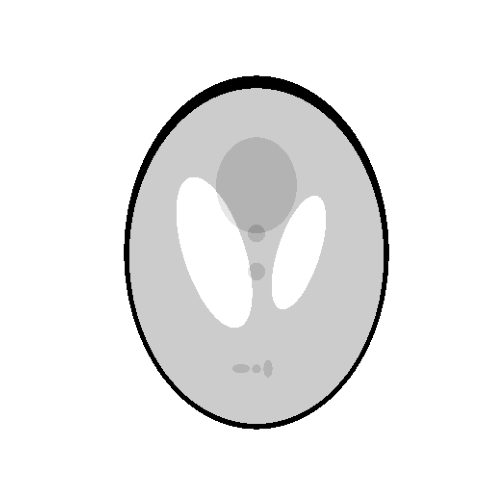
\includegraphics[width=0.18\textwidth]{phantom.png}}
    \subbottom[Original sinogram            \label{fig:ps:phantom_sinogram}]{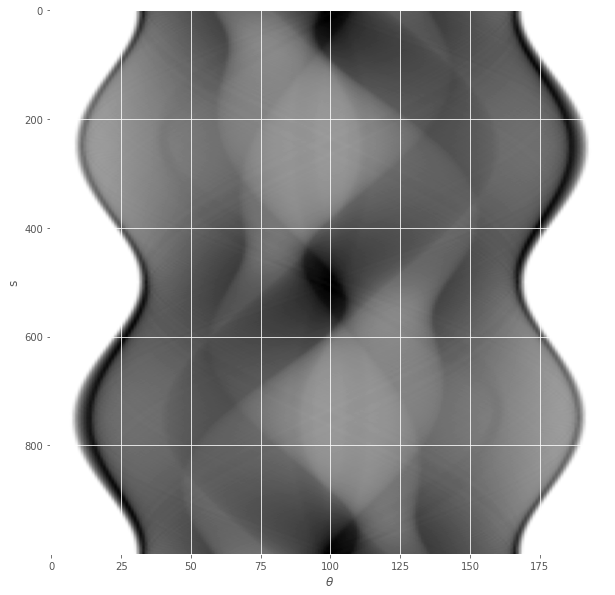
\includegraphics[width=0.18\textwidth]{phantom_sinogram.png}}
    \subbottom[Noisy sinogram               \label{fig:phantom_sinogram_noisy}]{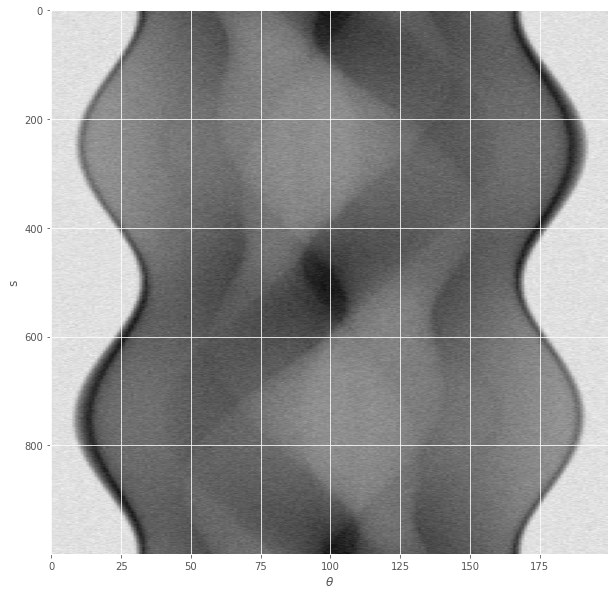
\includegraphics[width=0.18\textwidth]{phantom_sinogram_noisy.png}}
    \subbottom[2nd and 3rd smallest eigenvector of Graph Laplacian      \label{fig:phantom_second_third_evec}]{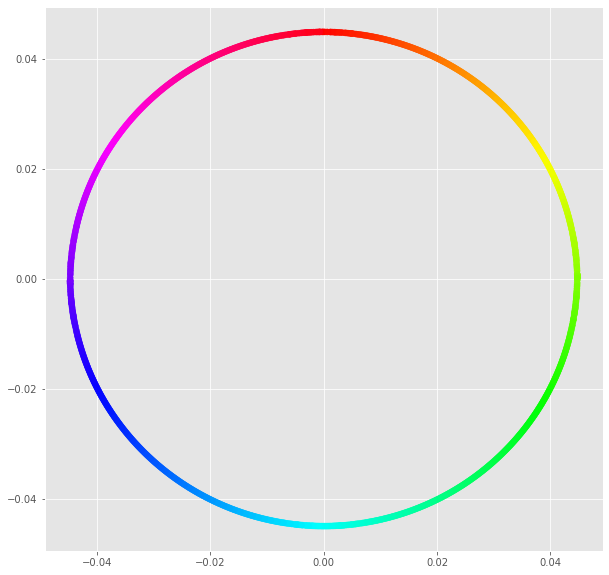
\includegraphics[width=0.18\textwidth]{phantom_second_third_evec.png}}
    \subbottom[2nd and 3rd smallest eigenvector of noisy Graph Laplacian\label{fig:phantom_second_third_evec_noisy}]{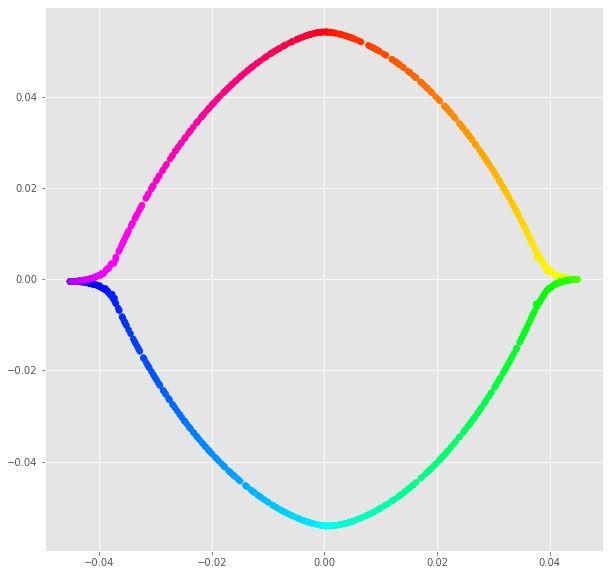
\includegraphics[width=0.18\textwidth]{phantom_second_third_evec_noisy.png}}
    \caption{Shepp-Logan phantom manifold}
\end{figure}

In Figure~\ref{fig:phantom_second_third_evec} the manifold calculated from the original Graph Laplacian
can be seen and it is a perfect circle. Next to it, in Figure~\ref{fig:phantom_second_third_evec_noisy}
the noisy version with $\sigma=2$ is plotted and the manifold is circle like but not at all like from the original one.

The more noise we add, the less the manifold looks like a circle. In Figure~\ref{fig:phantom_second_third_evec_noisy_high}
the manifold for $\sigma=100$ is plotted.

\begin{figure}[H]
    \centering
    \subtop[Highly noisy sinogram               \label{fig:phantom_sinogram_noisy_high}]{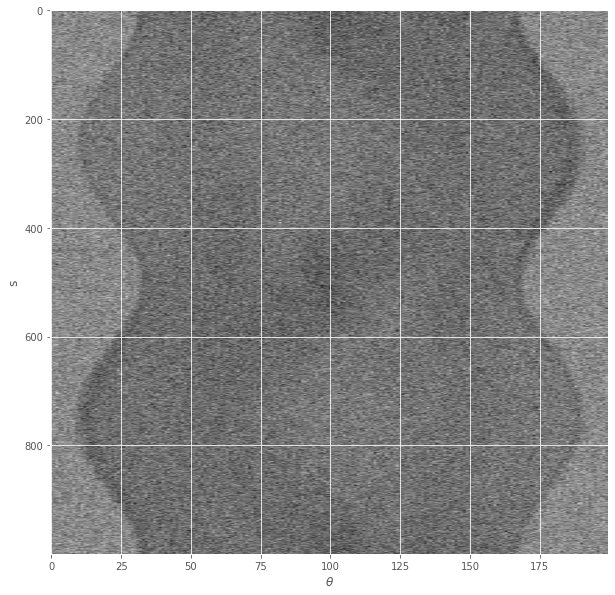
\includegraphics[width=0.4\textwidth]{phantom_sinogram_noisy_high.png}}
    \subtop[2nd and 3rd smallest eigenvector of Graph Laplacian      \label{fig:phantom_second_third_evec_noisy_high}]{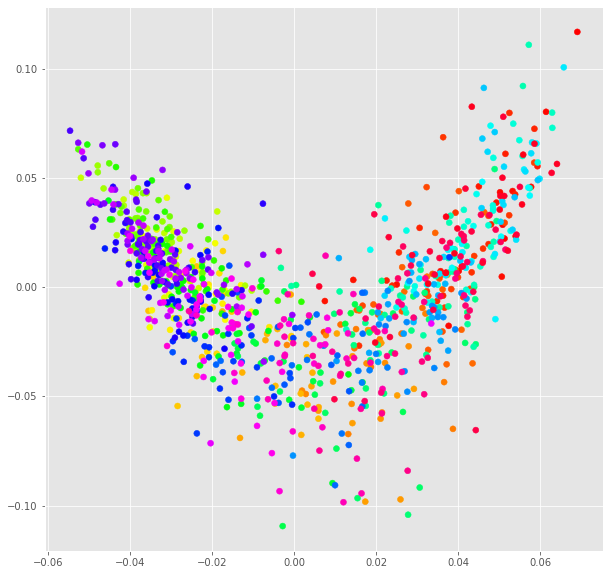
\includegraphics[width=0.4\textwidth]{phantom_second_third_evec_noisy_high.png}}
    \caption{Shepp-Logan phantom manifold for high noise level}
\end{figure}

In all the plots, knn-graph have been constructed with $k=10$. The showed example can be extended to 3D, where the underlying manifold corresponds to the sphere.
Again, the circle and sphere can be computed and for the none-noisy, the underlying manifold can be seen as known.


\section{Thesis problem}
During the Master Thesis, the reconstruction problem with unknown angles is considered. 
Moreover, the observed samples are considered to be noisy. 
The resulting proposed algorithm should work in the 2D and 3D scenario (classical tomography and cryo-Em).

The main idea is to exploit the fact, that the underlying manifold is known (circle in 2D and sphere in 3D). 
From our noisy observations, a manifold can be computed and compare it with the original manifold.
The comparison between the manifolds enables the possibility of a loss function and learning in general.

It is expected, that the folded spectrum \cite{foldedSpectrumMethod} introduced in section~\ref{sec:FoldedSpectrumMethod}
can be used to estimate the eigenvalues of the Graph Laplacian.
Further, as already mentioned in section~\ref{sec:wasserstein-metric}, the wasserstein metric is a good choice
as a loss function when it comes to dealing with data from a manifold distribution \cite{wassersteinGAN}, as in our case. 

The problem can be seen as Graph Denoising as observations are noisy and therefore, the proposed algorithm 
will denoise the graph based on the manifold assumption. 


\paragraph{Evaluation:}
During evaluation, 2D and 3D scenario will be considered. A first evaluation will be done on artificial constructed
toy-dataset. If time allows, real dataset from classical tomography and/or cryo-EM\footnote{https://www.ebi.ac.uk/emdb/} can be evaluated as well.
During evaluation, two baselines are considered which already solved the problem. The first one is a multi-frequency diffusion 
map approach\cite{multiDiffusionMaps, cryoEmMutliDM}, which aims to denoise cryo-EM images. 
Secondly, \cite{LaplaceRandomProjections} a Graph Laplacian approach solving classical tomography with random projection angles will be compare against.
The evaluation process is a first broad idea. Any adjustments in baseline papers or dataset are possible during 
the Master Thesis. The baseline papers are further addressed in the related work chapter~\ref{sec:relatedWork}
and detailed work packages are defined in chapter~\ref{sec:projectPlan}
